\documentclass[handout,nooutcomes]{ximera}
%% handout
%% space
%% newpage
%% numbers
%% nooutcomes

%I added the commands here so that I would't have to keep looking them up
%\newcommand{\RR}{\mathbb R}
%\renewcommand{\d}{\,d}
%\newcommand{\dd}[2][]{\frac{d #1}{d #2}}
%\renewcommand{\l}{\ell}
%\newcommand{\ddx}{\frac{d}{dx}}
%\everymath{\displaystyle}
%\newcommand{\dfn}{\textbf}
%\newcommand{\eval}[1]{\bigg[ #1 \bigg]}


\newcommand{\RR}{\mathbb R}
\renewcommand{\d}{\,d}
\newcommand{\dd}[2][]{\frac{d #1}{d #2}}
\renewcommand{\l}{\ell}
\newcommand{\ddx}{\frac{d}{dx}}
\newcommand{\dfn}{\textbf}
\newcommand{\eval}[1]{\bigg[ #1 \bigg]}

\usepackage{multicol}

\renewenvironment{freeResponse}{
\ifhandout\setbox0\vbox\bgroup\else
\begin{trivlist}\item[\hskip \labelsep\bfseries Solution:\hspace{2ex}]
\fi}
{\ifhandout\egroup\else
\end{trivlist}
\fi} %% we can turn off input when making a master document

\title{Recitation \#12 - 3.8 Implicit Differentiation}  

\begin{document}
\begin{abstract}		\end{abstract}
\maketitle

\section*{Warm up:} 
Explain why both the $x$-coordinate and the $y$-coordinate are generally needed to find the slope of the tangent line at a point on the graph of an implicitly defined function?
	\begin{freeResponse}
	If a function is defined \emph{implicitly} rather than \emph{explicitly}, then its graph will usually not pass the ``vertical line test".  So fixing a value for $x$ will not typically specify a unique point on the graph because there will be more than one corresponding $y$-value.  That is why you need to specify both the $x$ and the $y$ coordinate, to make sure that you are giving the coordinates for a unique point on the graph.
	\end{freeResponse}	
	
	
	
	
	

\section*{Group work:}



%problem 1
\begin{problem}
Consider the equation $x^2 + 4xy + 9y^2 = 9$

\begin{image}
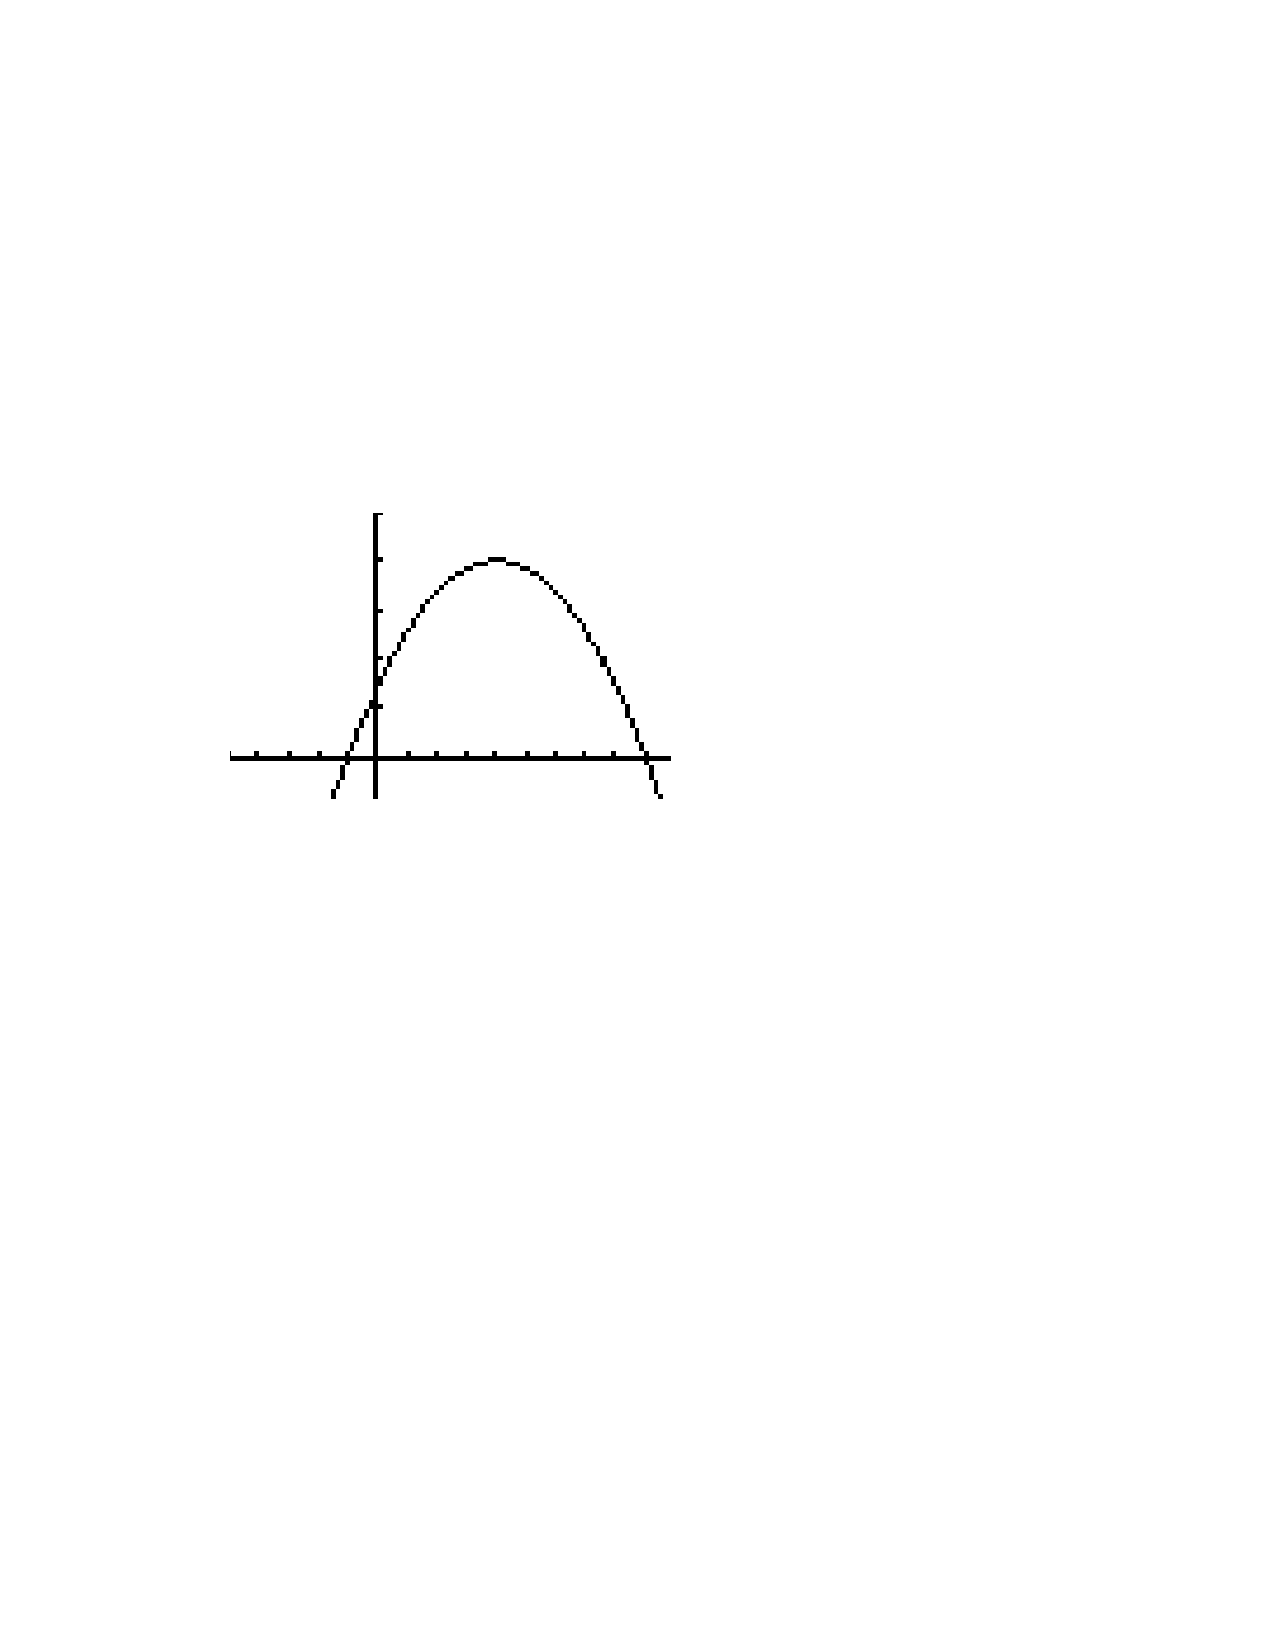
\includegraphics[trim= 140 450 290 220]{Figure1.pdf}
\end{image}

	\begin{enumerate}
	
	%part a
	\item  Find $\dd[y]{x}$.
		\begin{freeResponse}
		$$ \ddx(x^2 + 4xy + 9y^2) = \ddx(9) $$
		$$ 2x + \left(4y + 4x \dd[y]{x} \right) + 18 y \dd[y]{x} = 0 $$
		$$ 4x \dd[y]{x} + 18y \dd[y]{x} = -2x - 4y $$
		$$ (4x+18y) \dd[y]{x} = -2x-4y $$
		$$ \dd[y]{x} = \frac{-2x-4y}{4x+18y} $$
		provided that $4x+18y \neq 0$.
		\end{freeResponse}
		
		
		
%part b
	\item  Find the equation(s) of the tangent line(s) when $x=0$.  Draw the tangent line(s) on the above picture.
		\begin{freeResponse}
		Plugging into the original equation, we see that when $x=0$ we have that 
		$$ 0^2 + 4(0)y + 9y^2 = 9 \qquad \Longrightarrow \qquad y^2 = 1 \qquad \Longrightarrow \qquad y = \pm 1 $$
		
		Then,
		$$\eval{\dd[y]{x}}_{(0,1)} = \frac{-4}{18} = -\frac{2}{9}$$
		$$\eval{\dd[y]{x}}_{(0,-1)} = \frac{4}{-18} = -\frac{2}{9} $$
		
		So there are two tangent lines to the graph of the solution set to the given equation when $x=0$.  The two solutions are $(0,1)$ and $(0,-1)$, and the tangent lines at both points have slope $-\frac{2}{9}$.  Thus, the equations to the two tangent lines are
		$$ y - 1 = -\frac{2}{9}(x-0)  \qquad \Longrightarrow \qquad y = -\frac{2}{9}x + 1 $$
		$$ y + 1 = -\frac{2}{9}(x-0) \qquad \Longrightarrow \qquad y = -\frac{2}{9}x - 1 $$
		\end{freeResponse}
		
		
		
%part c
	\item  Find the point(s) where the tangent line is horizontal.  Draw the point(s) and line(s) on the above picture.
		\begin{freeResponse}
		A line is horizontal if and only if its slope is 0.  So we are looking for the points $(x_0,y_0)$ such that $\eval{\dd[y]{x}}_{(x_0,y_0)} = 0$.  So we solve:
		$$ \frac{-2x-4y}{4x+18y} = 0\qquad \Longrightarrow \qquad -2x - 4y = 0 \qquad \Longrightarrow \qquad x=-2y$$
		
		But we also need the point to satisfy the given equation.  So, letting $x=-2y$, we solve:
		$$x^2 + 4xy + 9y^2 = 9 $$
		$$ (-2y)^2 + 4(-2y)y + 9y^2 = 9 $$
		$$ 4y^2 - 8y^2 + 9y^2 = 9 $$
		$$ 5y^2 = 9 $$
		$$ y^2 = \frac{9}{5} $$
		$$ y = \pm \frac{3}{\sqrt{5}} $$
		
		So there exists two solutions to the given equation where the tangent line to the graph has 0 slope.  Those two points are $\left( -\frac{6}{\sqrt{5}}, \frac{3}{\sqrt{5}} \right)$ and $\left( \frac{6}{\sqrt{5}}, - \frac{3}{\sqrt{5}} \right)$.
		\end{freeResponse}
		
		
		
	\end{enumerate}
			
			
	
\end{problem}
















%problem 2
\begin{problem}
Find the slope of the tangent line (at any point $(x,y)$) to the graph of the solution set to the given equation

	\begin{enumerate}
	
	%part a
	\item  $e^{x^2 y^3} - 5x + 7y = 36$
			\begin{freeResponse}
			$$ e^{x^2 y^3} \left( 2xy^3 + x^2 (3y^2)\dd[y]{x} \right) - 5 + 7\dd[y]{x} = 0 $$
			$$ 2xy^3 e^{x^2y^3} + 3x^2y^2e^{x^2y^3}\dd[y]{x} - 5 + 7\dd[y]{x} = 0 $$
			$$ 3x^2y^2e^{x^2y^3}\dd[y]{x} + 7\dd[y]{x} = -2xy^3 e^{x^2y^3} + 5 $$
			$$ \left( 3x^2y^2e^{x^2y^3} + 7 \right) \dd[y]{x} = -2xy^3 e^{x^2y^3} + 5 $$
			$$  \dd[y]{x} = \frac{-2xy^3 e^{x^2y^3} + 5}{3x^2 y^2 e^{x^2y^3} + 7} $$
			\end{freeResponse}
			
			
			
	%part b
	\item  $7 = 22 \tan(y) + \frac{4}{x} - \frac{7}{y}$
			\begin{freeResponse}
			$$ 0 = 22 \sec^2 (y) \dd[y]{x} - \frac{4}{x^2} + \frac{7}{y^2} \dd[y]{x} $$
			$$ 22 \sec^2(y) \dd[y]{x} + \frac{7}{y^2} \dd[y]{x} = \frac{4}{x^2} $$
			$$ \dd[y]{x} = \frac{\frac{4}{x^2}}{22 \sec^2(y) + \frac{7}{y^2}} $$
			\end{freeResponse}
			
			
			
	%part c
	\item  $\cos(xy) - x^3 = 5y^3$
			\begin{freeResponse}
			$$ -\sin(xy) \cdot \left(y + x \dd[y]{x} \right) - 3x^2 = 15y^2 \dd[y]{x} $$
			$$ -y \sin(xy) - x \sin(xy) \dd[y]{x} - 3x^2 = 15y^2 \dd[y]{x} $$
			$$ x \sin(xy) \dd[y]{x} + 15y^2 \dd[y]{x} = -y \sin(xy) - 3x^2 $$
			$$ \dd[y]{x} = \frac{-y \sin(xy) - 3x^2}{x \sin(xy) + 15y^2} $$
			
			Provided that $x \sin(xy) + 15y^2 \neq 0$.  It is worth pointing out that this condition was not necessary for parts (a) and (b) because the denominator of those solutions cannot be $0$.  
			\end{freeResponse}
			
			
			
	\end{enumerate}
			
			
			
		
\end{problem}
	
	
	
	
	
	
	
	
			
			

%problem 3			
\begin{problem}
If $9x^2 + y^2 = 9$, find $\dd[^2 y]{x^2}$ as a function of $x$ and $y$.
		\begin{freeResponse}
		$18x + 2y \dd[y]{x} = 0 \qquad \Longrightarrow \qquad \dd[y]{x} = - \frac{18x}{2y} = - \frac{9x}{y}$.
		
		Then,
		$$ \dd[^2y]{x^2} = \ddx \dd[y]{x} = \ddx \left( - \frac{9x}{y} \right) = - \frac{(y)(9) - (9x)(\dd[y]{x} )}{y^2} = \frac{9x\dd[y]{x} - 9y}{y^2}. $$
		
		This is not a sufficient answer to the question since $\dd[y]{x}$ is a part of the solution.  But we know that $\dd[y]{x} = -\frac{9x}{y}$, and so we can substitute to get
		
		$$ \dd[^2y]{x^2} = \frac{(9x) \left(- \frac{9x}{y} \right) - 9y}{y^2} = \frac{-81x^2 - 9y^2}{y^3}. $$
		
		Provided that $y \neq 0$.  
		\end{freeResponse}
		
		
		
	
		
\end{problem}
















	
	
	
	
	
	
	
	
	

	










								
				
				
	














\end{document} 


















